\subsection{Testing for Reflected Cross Site Scripting - OTG-INPVAL-001} \label{OTG-INPVAL-001}

\begin{longtable}[l]{ p{2.3cm} | p{.79\linewidth} }\hline
    & \textbf{Online Banking}
    \hfill CVSS Score: 0.0 \progressbar[filledcolor=Green]{0.0}
    \\ \hline
    \textbf{Observation} & It has been found that Reflected Cross Site Scripting is possible in the application in the \code{Make Payment} interface. \\
    \textbf{Discovery} & Manual inspection of code revealed usage of functions such as \code{htmlspecialchars}, \code{filter\_var} and \code{preg\_match} for input sanitization; leading to HTML tags being rendered as plain text. However, while rendering output, absence of sanitization leads to this issue. Usage of \code{echo \$\_POST['receipt'];} was found at multiple locations in code. Refer to \ref{code:reflected_xss} for the related code.
    This was confirmed by a black box test. See \ref{fig:OTG-INPVAL-001} for an example of this vulnerability.\\
    \textbf{Likelihood} & Likelihood is low as exploitation of this vulnerability requires some technical skills. Moreover, an attacker can only perform this attack if he/she has access to user credentials. \\
    \textbf{Impact} & Impact is none as exploitation of this vulnerability does not affect other users. \\
    \textbf{Recommen\-dations} & It is recommended to properly sanitize output before generating web content for the user. \\ \hline
    \textbf{CVSS} &
        \begin{tabular}[t]{@{}l | l}
            Attack Vector           & \textcolor{red}{Network} \\
            Attack Complexity       & \textcolor{red}{Low}\\
            Privileges Required     & \textcolor{red}{None}\\
            User Interaction        & \textcolor{red}{None} \\
            Scope                   & \textcolor{Green}{Unchanged} \\
            Confidentiality Impact  & \textcolor{Green}{None} \\
            Integrity Impact        & \textcolor{Green}{None} \\
            Availability Impact     & \textcolor{Green}{None}
        \end{tabular}
    \\ \hline
\end{longtable}

\clearpage
\begin{longtable}[l]{ p{2.3cm} | p{.79\linewidth} }\hline
    & \textbf{SecureBank}
    \\ \hline
    \textbf{Observation} & It has been verified that Reflected Cross Site Scripting is not possible. All the URLs where we tried to append script and HTML tags returned the response as 404. \\
    \textbf{Discovery} & Manual inspection of code revealed usage of functions such as \code{htmlspecialchars}, \code{filter\_var} and \code{preg\_match} for input sanitization; leading to HTML tags being rendered as plain text. \\
    \textbf{Likelihood} & N/A \\
    \textbf{Impact} & N/A \\
    \textbf{Recommen\-dations} & N/A \\ \hline
    \textbf{CVSS} & N/A
    \\ \hline
\end{longtable}

\subsubsection{Comparison}
SecureBank is better than Online Banking as it is completely safe from XSS attacks.

\begin{lstlisting}[caption={PHP code for rendering content in Make Payment page from online.php}\label{code:reflected_xss}, language=PHP, basicstyle=\footnotesize, frame=single, captionpos=t, linewidth=.9\textwidth, xleftmargin=.12\textwidth]
    <div class="form-group">
        <input type="text" name="receipt" value="<?php
         echo $_POST['receipt']; ?>"
         class="form-control" id="receipt" placeholder="Receipt"
         required>
    </div>
    <div class="form-group">
        <input type="text" name="amount" value="<?php
         echo $_POST['amount']; ?>"
         class="form-control" id="amount"  placeholder="Amount in euro"
         required  aria-required="true" pattern="[0-9]+"
         title="Please, input the field with digits">
    </div>
    <div class="form-group">
        <textarea class="form-control black-field" name="purpose"
         class="form-control" id="purpose"  placeholder="Purpose"
         rows="2" required aria-required="true"><?php
         echo $_POST['purpose']; ?></textarea>
    </div>
    <div class="form-group">
        <input type="text" name="trancode" value="<?php
         echo $_POST['trancode']; ?>"
         class="form-control" placeholder="TAN" id="TAN" required>
    </div>
\end{lstlisting}

\begin{figure}[ht]
	\centering
		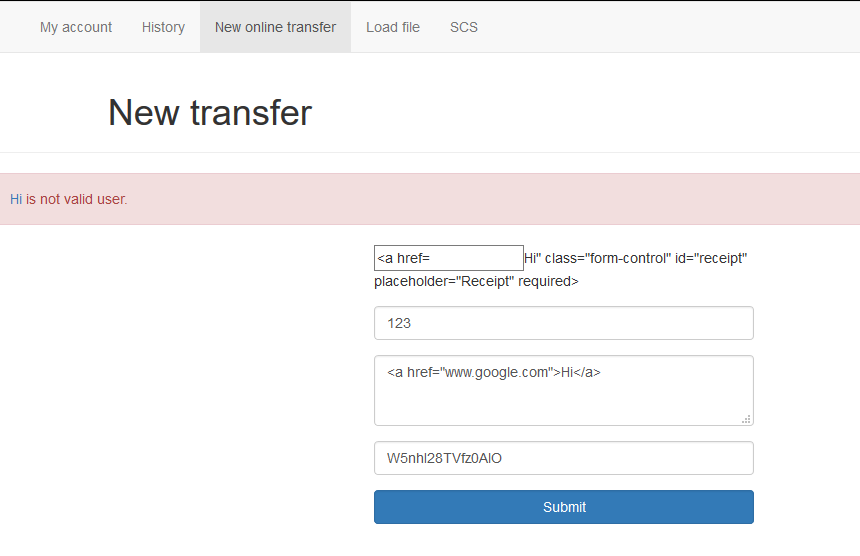
\includegraphics[width=.8\linewidth]{figures/OTG-INPVAL-001.png}
		\caption{Reflected XSS in Make Payment page}
	\label{fig:OTG-INPVAL-001}
\end{figure}

\clearpage